\newpage

\section{Własności}

\subsection{Siarczek galu}
Struktura pasmowa i przerwa energetyczna to są kluczowe parametry dla półprzewodników chalkogenowych. \textit{Chalkogenki} – nieorganiczne związki chemiczne, w których anionami są chalkogeny, tj. siarczki, selenki i telurki. Przykładowymi chalkogenkami są związki $\mathbf{GaS}$, $\mathbf{Ga_{2}S_{3}}$, $\mathbf{GaSe}$, $\mathbf{Ga_{2}Se_{3}}$, które należą do związków III-VI (III: \textbf{In}, \textbf{Ga} i VI: \textbf{S}, \textbf{Se}, \textbf{Te}) grupy chemicznej. Związek $\mathbf{Ga_{2}S_{3}}$ jest ważnym członkiem związków III-VI , który może posiadać najszerszą lukę w zespole. Nieścisłość pomiędzy atomami III i VI grup powoduje, że związek ma różne stechiometrie, zróżnicowane fazy krystaliczne i różne formy sieci.[2][3]

$\mathbf{GaSe}$ i $\mathbf{GaS}$ mogą krystalizować się w sześciakątnej strukturze warstwowej, ale w tych związkach warstwy różnie układają się w stos. $\mathbf{GaSe}$ posiada prostą przerwę energetyczną wynoszącą około 2 eV. Podczas gdy materiał $\mathbf{GaS}$ staje się przewodnikiem ze skośną przerwą energetyczną o wartości 2.53 eV.[6]

$\mathbf{Ga_{2}Se_{3}}$ może posiadać wadliwą strukturę blendy cynkowej, w której 1/3 miejsc kationowych jest pusta (położenie pustych miejsc jest losowe w siatce krystalicznej) jest to oczywiście zdefektowany półprzewodnik z prostą przerwą energetyczną o wartości 2-2.4eV.[7]

Chalkogenki $\mathbf{GaSe}$, $\mathbf{GaS}$, $\mathbf{Ga_{2}Se_{3}}$ mają wartości przerwy energetycznej poniżej 2.55 eV. które mogą być zakatologowane do materiałów w zakresie widzialnyma, ale nie do zastosowań w zakresie UV jak związek $\mathbf{Ga_{2}S_{3}}$[8][9]

Siarczek galu występuje w dwóch postaciach:
\begin{itemize}
	\item Siarczek galu(II) - $\mathbf{GaS}$
	\item Siarczek galu(III) - $\mathbf{Ga_{2}S_{3}}$
\end{itemize}
%grupa przestrzenna $\mathbf{P\;6_{3}/mmc}$
$\mathbf{GaS}$ tworzy bezbarwne lub żółte kryształki układu heksagonalnego. Kryształ siarczku galu $\mathbf{(GaS)}$ należy do rodziny półprzewodników warstwowych III-VI. Krystalizuje się w sześciokątnej strukturze o parametrach sieci $a = 0,3578$ i $c = 1,547$ nm. Każda warstwa w strukturze krystalicznej składa się z dwóch atomów galu i dwóch atomów siarki ułożonych w stos wzdłuż osi $c$ z powtarzającą się jednostką $\mathbf{S-Ga-Ga-S}$.[11][12][13]
\begin{figure}[H]
	\begin{center}
		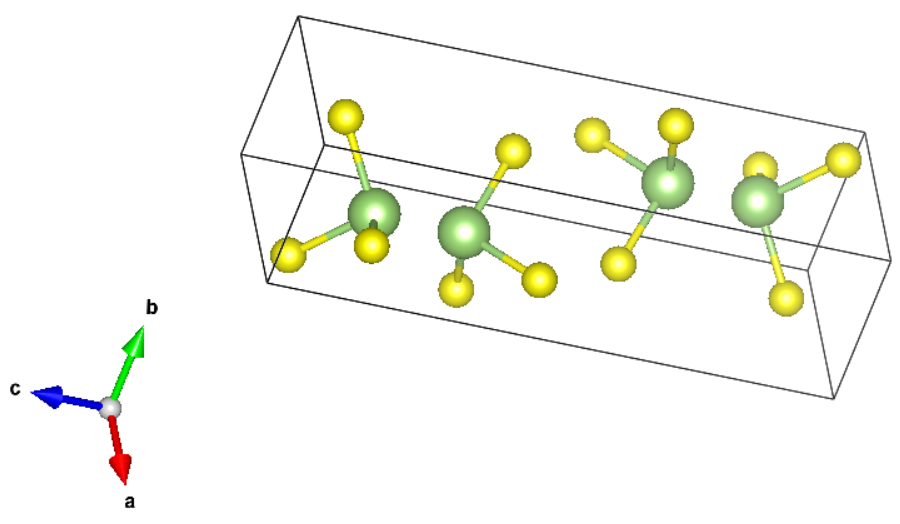
\includegraphics[width=0.85\linewidth]{Wlasciwosci/GaS/GaS_vesta.png}
		\caption{Schematyczna reprezentacja struktury krystalicznej $\mathbf{GaS}$. Przygotowano używając oprogramowania VESTA.[5]}
	\end{center}
\end{figure}

W kryształach $\mathbf{GaS}$ dominują słabe siły van der Waalsa w oddziaływaniach międzywarstwowych. Silne kowalencyjne siły dominują w oddziaływaniach wewnątrzwarstwowych.
$\mathbf{GaS}$ to półprzewodnik szerokopasmowy, który jest obiecującym materiałem. Skośna przerwa energetyczna wynosi $2.5eV$, a prosta wynosi $2.95eV$. Materiał umożliwia
wytwarzanie niebieskich urządzeń emitujących światło [1].

$\mathbf{Ga_{2}S_{3}}$ jest również półprzewodnikiem zdefektowanym z powodu niedopasowania $\mathbf{Ga}$ – III i $\mathbf{S}$ - VI. Jedna trzecia miejsc kationowych, czyli pozycji galowych nie jest zajęte. Występują luki kationowe, które znacznie wpływają na właściwości fizyczne tego materiału i jego obszar zastosowań. Może mieć następne struktury krystaliczne: jednoskośna, heksagonalna, kubiczna.

\begin{enumerate}
	\item \textit{Faza $\alpha'$-$\mathbf{Ga_{2}S_{3}}$} \\
	Najbardziej stabilną fazą związku $\mathbf{Ga_{2}S_{3}}$ jest faza $\alpha'$-$\mathbf{Ga_{2}S_{3}}$.
	\begin{itemize}
		\item Ma jednoskośny układ krystalograficzny;
		\item Związek $\alpha'$-$\mathbf{Ga_{2}S_{3}}$ ma prostą przerwę energetyczną o wartości 3.05 - 3.30 eV \footnote{W zależności od źródła.} i skośną przerwę energetyczną o wartości 3.4 eV.
		\item Wyhodowane kryształki są jasnożółte lub przezroczyste. Powodem występowania żółtego koloru w tym półprzewodniku, gdzie przerwa energetyczna ma energię większą niż najbardziej energetyczny foton światła widzialnego, jest obecność luk kationowych. Luki w pasmie energetycznym zlokalizowane na poziomie 0.8 - 0.9 eV wyżej od najwyższego punktu pasma walencyjnego. Te luki tworzą pułapki elektronowe. Elektrony które przechodzą z pasma przewodnictwa do tych pułapek emitują fotony o energii 2.15 - 2.25 eV co odpowiada światłu żółtemu.
		\item Może posiadać dwie grupy przestrzenne. Parametry komórki elementarnej dla tego materiału w zależności od grupy przestrzennej wynoszą:
		\begin{itemize}
			\item Grupa przestrzenna $Cc$ - $a=1.111\;nm$, $b=0.640\;nm$, $c=0.702\;nm$, $\beta=121.17^{\circ}$;
			\item Grupa przestrzenna $Bb$ -  $a=1.109\;nm$, $b=0.958\;nm$, $c=0.640\;nm$, $\beta=141.15^{\circ}$;
		\end{itemize}
	\end{itemize} 
	
	\begin{figure}[H]
		\begin{center}
			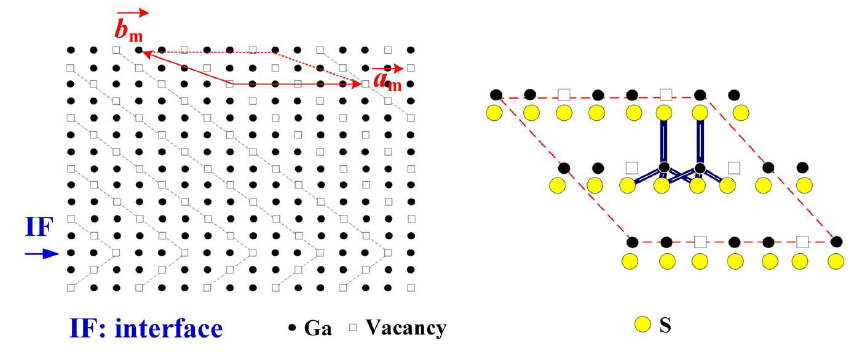
\includegraphics[width=1.0\linewidth]{Wlasciwosci/Przekroj_Ga2S3.png}
			\caption{Na lewym rysunku przedstawiono zdefektowaną sieć krystaliczną w płaszczyźnie prostopadłej do osi c dla związku $\alpha'$-$\mathbf{Ga_{2}S_{3}}$. Kationowe luki tworzą interfejs. Na prawym rysunku pokazano sposób ułożenia i wiązania atomów. Cztery aniony $\mathbf{S}$ w wierzchołkach czworościanu i w środku jeden kation $\mathbf{Ga}$ lub luka.[6]}
		\end{center}
	\end{figure}
	
	\begin{figure}[H]
		\begin{minipage}[h]{0.47\linewidth}
			\center{\includegraphics[width=1\linewidth]{Wlasciwosci/Ga2S3/Cc/Ga2S3_a.png}} a) \\
		\end{minipage}
		\hfill
		\begin{minipage}[h]{0.47\linewidth}
			\center{\includegraphics[width=1\linewidth]{Wlasciwosci/Ga2S3/Cc/Ga2S3_b.png}} \\b)
		\end{minipage}
		\vfill
		\begin{minipage}[h]{0.47\linewidth}
			\center{\includegraphics[width=1\linewidth]{Wlasciwosci/Ga2S3/Cc/Ga2S3_c.png}} c) \\
		\end{minipage}q
		\hfill
		\begin{minipage}[h]{0.47\linewidth}
			\center{\includegraphics[width=1\linewidth]{Wlasciwosci/Ga2S3/Cc/Ga2S3_vesta.png}} d) \\
		\end{minipage}
		\caption{Komórka elementarna dla $\alpha'$-$\mathbf{Ga_{2}S_{3}}$. Grupa przestrzenna $Cc$. Przygotowano używając oprogramowanie VESTA.[5]}
		\begin{minipage}[h]{0.47\linewidth}
			\center{\includegraphics[width=1\linewidth]{Wlasciwosci/Ga2S3/Bb/Ga2S3_a.png}} a) \\
		\end{minipage}
		\hfill
		\begin{minipage}[h]{0.47\linewidth}
			\center{\includegraphics[width=1\linewidth]{Wlasciwosci/Ga2S3/Bb/Ga2S3_b.png}} \\b)
		\end{minipage}
		\vfill
		\begin{minipage}[h]{0.47\linewidth}
			\center{\includegraphics[width=1\linewidth]{Wlasciwosci/Ga2S3/Bb/Ga2S3_c.png}} c) \\
		\end{minipage}
		\hfill
		\begin{minipage}[h]{0.47\linewidth}
			\center{\includegraphics[width=1\linewidth]{Wlasciwosci/Ga2S3/Bb/Ga2S3_vesta.png}} d) \\
		\end{minipage}
		\caption{Komórka elementarna dla $\alpha'$-$\mathbf{Ga_{2}S_{3}}$. Grupa przestrzenna $Bb$. Przygotowano używając oprogramowanie VESTA.[5]}
	\end{figure}
	
	\item Fazy $\alpha$-$Ga_{2}S_{3}$ ma grupę przestrzenną $P6_1$. Ta faza ma sześciokątny układ krystalograficzny. Parametry komórki elementarnej $a=0.639\;nm$, $c=1.804\;nm$.
	
	\begin{figure}[H]
		\begin{minipage}[h]{0.47\linewidth}
			\center{\includegraphics[width=1\linewidth]{Wlasciwosci/Ga2S3/alfa/Ga2S3_a.png}} a) \\
		\end{minipage}
		\hfill
		\begin{minipage}[h]{0.47\linewidth}
			\center{\includegraphics[width=1\linewidth]{Wlasciwosci/Ga2S3/alfa/Ga2S3_b.png}} \\b)
		\end{minipage}
		\vfill
		\begin{minipage}[h]{0.47\linewidth}
			\center{\includegraphics[width=1\linewidth]{Wlasciwosci/Ga2S3/alfa/Ga2S3_c.png}} c) \\
		\end{minipage}q
		\hfill
		\begin{minipage}[h]{0.47\linewidth}
			\center{\includegraphics[width=1\linewidth]{Wlasciwosci/Ga2S3/alfa/Ga2S3_vesta.png}} d) \\
		\end{minipage}
		\caption{Komórka elementarna dla $\alpha$-$\mathbf{Ga_{2}S_{3}}$. Przygotowano używając oprogramowanie VESTA.[5]}
	\end{figure}

	\item \textit{Faza $\beta$-$\mathbf{Ga_{2}S_{3}}$} \\
	Ta faza jest nazywana fazą $\beta$, z sześciokątnym układem krystalograficznym. Grupa przestrzenna $P6_{3}mc$ Parametry komórki elementarnej: $a=0.368\;nm$,  $c=0.602\;nm$. Faza $\beta$ związku $\mathbf{Ga_{2}S_{3}}$ ma najmniejszą przerwę energetyczną dla tego materiału 2.48 eV.
	
	\begin{figure}[H]
		\begin{minipage}[h]{0.47\linewidth}
			\center{\includegraphics[width=1\linewidth]{Wlasciwosci/Ga2S3/beta/Ga2S3_a.png}} a) \\
		\end{minipage}
		\hfill
		\begin{minipage}[h]{0.47\linewidth}
			\center{\includegraphics[width=1\linewidth]{Wlasciwosci/Ga2S3/beta/Ga2S3_b.png}} \\b)
		\end{minipage}
		\vfill
		\begin{minipage}[h]{0.47\linewidth}
			\center{\includegraphics[width=1\linewidth]{Wlasciwosci/Ga2S3/beta/Ga2S3_c.png}} c) \\
		\end{minipage}q
		\hfill
		\begin{minipage}[h]{0.47\linewidth}
			\center{\includegraphics[width=1\linewidth]{Wlasciwosci/Ga2S3/beta/Ga2S3_vesta.png}} d) \\
		\end{minipage}
		\caption{$\beta$-$\mathbf{Ga_{2}S_{3}}$. Przygotowano używając oprogramowanie VESTA.[5]}
	\end{figure}

	\item \textit{Faza $\gamma$-$\mathbf{Ga_{2}S_{3}}$} \\
	Faza z grupą przestrzenna $F-43m$. To jest niskotemperaturowa faza. Kryształki $\gamma$-$\mathbf{Ga_{2}S_{3}}$ są białego koloru. Przerwa energetyczna wynosi 2.96 eV. Parametry komórki elementarnej: $a=0.517\;nm$.
	\begin{center}
		\begin{figure}[H]
			\begin{minipage}[h]{0.47\linewidth}
				\center{\includegraphics[width=0.8\linewidth]{Wlasciwosci/Ga2S3/gamma/Ga2S3_vesta.png}} a) \\
			\end{minipage}
			\hfill
			\begin{minipage}[h]{0.47\linewidth}
				\center{\includegraphics[width=0.8\linewidth]{Wlasciwosci/Ga2S3/gamma/Ga2S3_a.png}} \\b)
			\end{minipage}
			\caption{Komórka elementarna dla $\gamma$-$\mathbf{Ga_{2}S_{3}}$. Przygotowano używając oprogramowanie VESTA.[5]}
		\end{figure}
	\end{center}
	
\end{enumerate}

Poniżej została przedstawiona tabela, w której zostały zebrane informację o czterech fazach krystalicznych materiału $\mathbf{Ga_{2}S_{3}}$:
\begin{table}[H]
	\begin{tabular}{|c|c|c|c|c|}
		\hline
		\multicolumn{1}{|l|}{\textbf{Nazwa}} & \textbf{\begin{tabular}[c]{@{}c@{}}Układ \\ krystalograficzny\end{tabular}} & \textbf{\begin{tabular}[c]{@{}c@{}}Grupa\\ przestrzenna\end{tabular}} & \textbf{Typ struktury}                                            & \textbf{\begin{tabular}[c]{@{}c@{}}Parametry sieci\\ krystalicznej\end{tabular}} \\ \hline
		$\alpha$-$\mathbf{Ga_{2}S_{3}}$                              & Heksagonalny                                                               & $P6_{1}$                       & \begin{tabular}[c]{@{}c@{}}Superstruktura \\ wurcytu\end{tabular} & $a=0.639\;nm$,$c=1.804\;nm$                                                                   \\ \hline
		\multirow{2}{*}{$\alpha'$-$\mathbf{Ga_{2}S_{3}}$}            & \multirow{2}{*}{Jednoskośny}                                                & $Cc$                          & \begin{tabular}[c]{@{}c@{}}Superstruktura\\ $\alpha$-$\mathbf{Ga_{2}S_{3}}$\end{tabular}  & 
		\begin{tabular}[c]{@{}c@{}}$a=1.111\;nm$, $b=0.640\;nm$,\\ $c=0.702\;nm$,$\beta=121.17^{\circ}$\end{tabular}                                                                            \\ \cline{3-5} 
		&                                                                             & $Bb$                          & \begin{tabular}[c]{@{}c@{}}Superstruktura\\ $\alpha$-$\mathbf{Ga_{2}S_{3}}$\end{tabular}  & 	
		\begin{tabular}[c]{@{}c@{}}$a=1.109\;nm$, $b=0.958\;nm$,\\ $c=0.640\;nm$, $\beta=141.15^{\circ}$\end{tabular}                                                                            \\ \hline
		$\beta$-$\mathbf{Ga_{2}S_{3}}$                              & Sześciokątny                                                                & $P6_{3}mc$                     & Wurcyt                                                            & $a=0.368\;nm$,                                                                                           $c=0.602\;nm$                                                                              \\ \hline
		$\gamma$-$\mathbf{Ga_{2}S_{3}}$                              & Sześcienny                                                                  & $F$-$43m$                       & Blenda cynkowa                                                    & $a=0.517\;nm$                                                                            \\ \hline
	\end{tabular}
	\caption{Wszystkie fazy krystaliczne $\mathbf{Ga_{2}S_{3}}$.[27]}
\end{table}

Główne piki na widmie rentgenowskim dla każdej z faz występują pod tymi samymi kątami, jedynie intensywności mają różne. To oznacza że jeżeli Faza kubiczna $\gamma$-$\mathbf{Ga_{2}S_{3}}$ ma strukturę blendy cynkowej $\mathbf{ZnS}$ ze zdefektowaną podsiecią kationową, to i każda z faz też będzie miała zdefektowaną podsieć kationową.

Widma ramanowskie i widma rentgenowskie są prawie takie same dla każdej z faz $\mathbf{Ga_{2}S_{3}}$. Dla tego informacje o strukturze tego materiału w literaturze są niejednoznaczne i często niespójne. Widmo polaryzacyjne dla tego materiału może być dobrym parametrem dla określenia fazy $\mathbf{Ga_{2}S_{3}}$. W tej pracy zajmuję się badaniem widma polaryzacyjnego dla $\alpha'$-$\mathbf{Ga_{2}S_{3}}$ która ma grupę przestrzenną $Cc$.

\begin{figure}[H]
	\begin{minipage}[h]{0.47\linewidth}
		\center{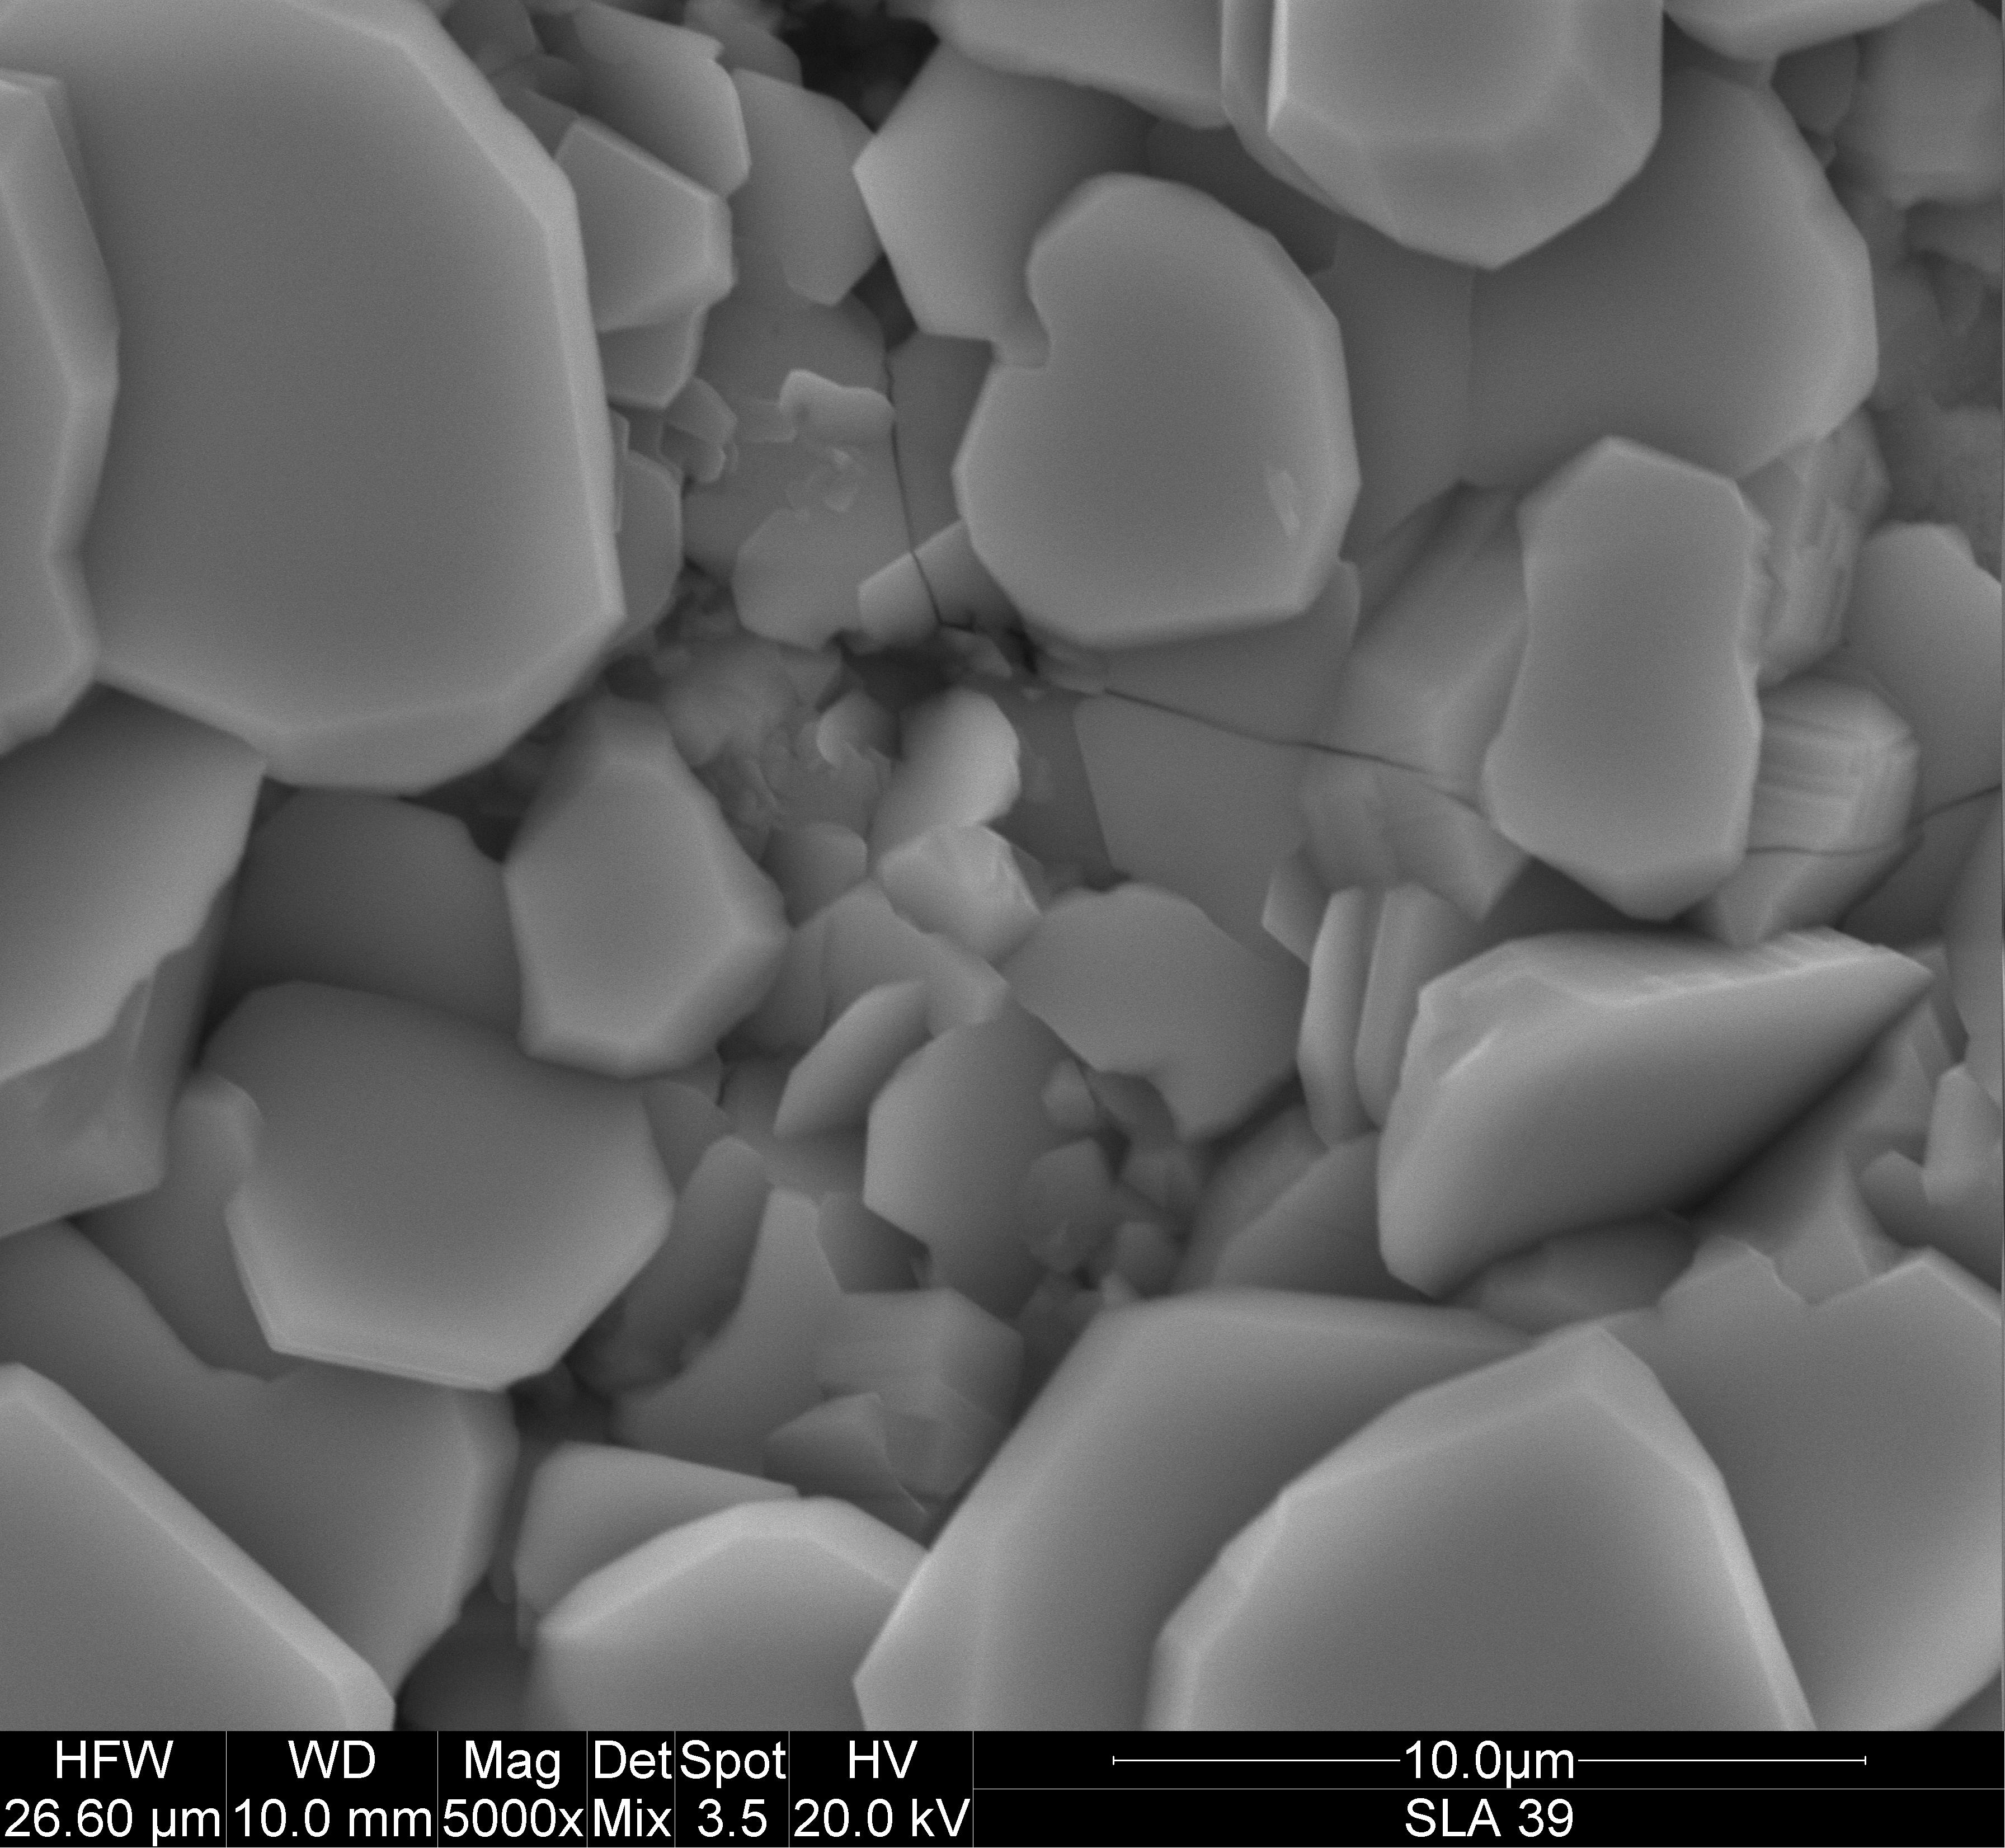
\includegraphics[width=0.8\linewidth]{Wlasciwosci/SLA39_MIX_5000.jpg}} \\a) 
	\end{minipage}
	\hfill
	\begin{minipage}[h]{0.47\linewidth}
		\center{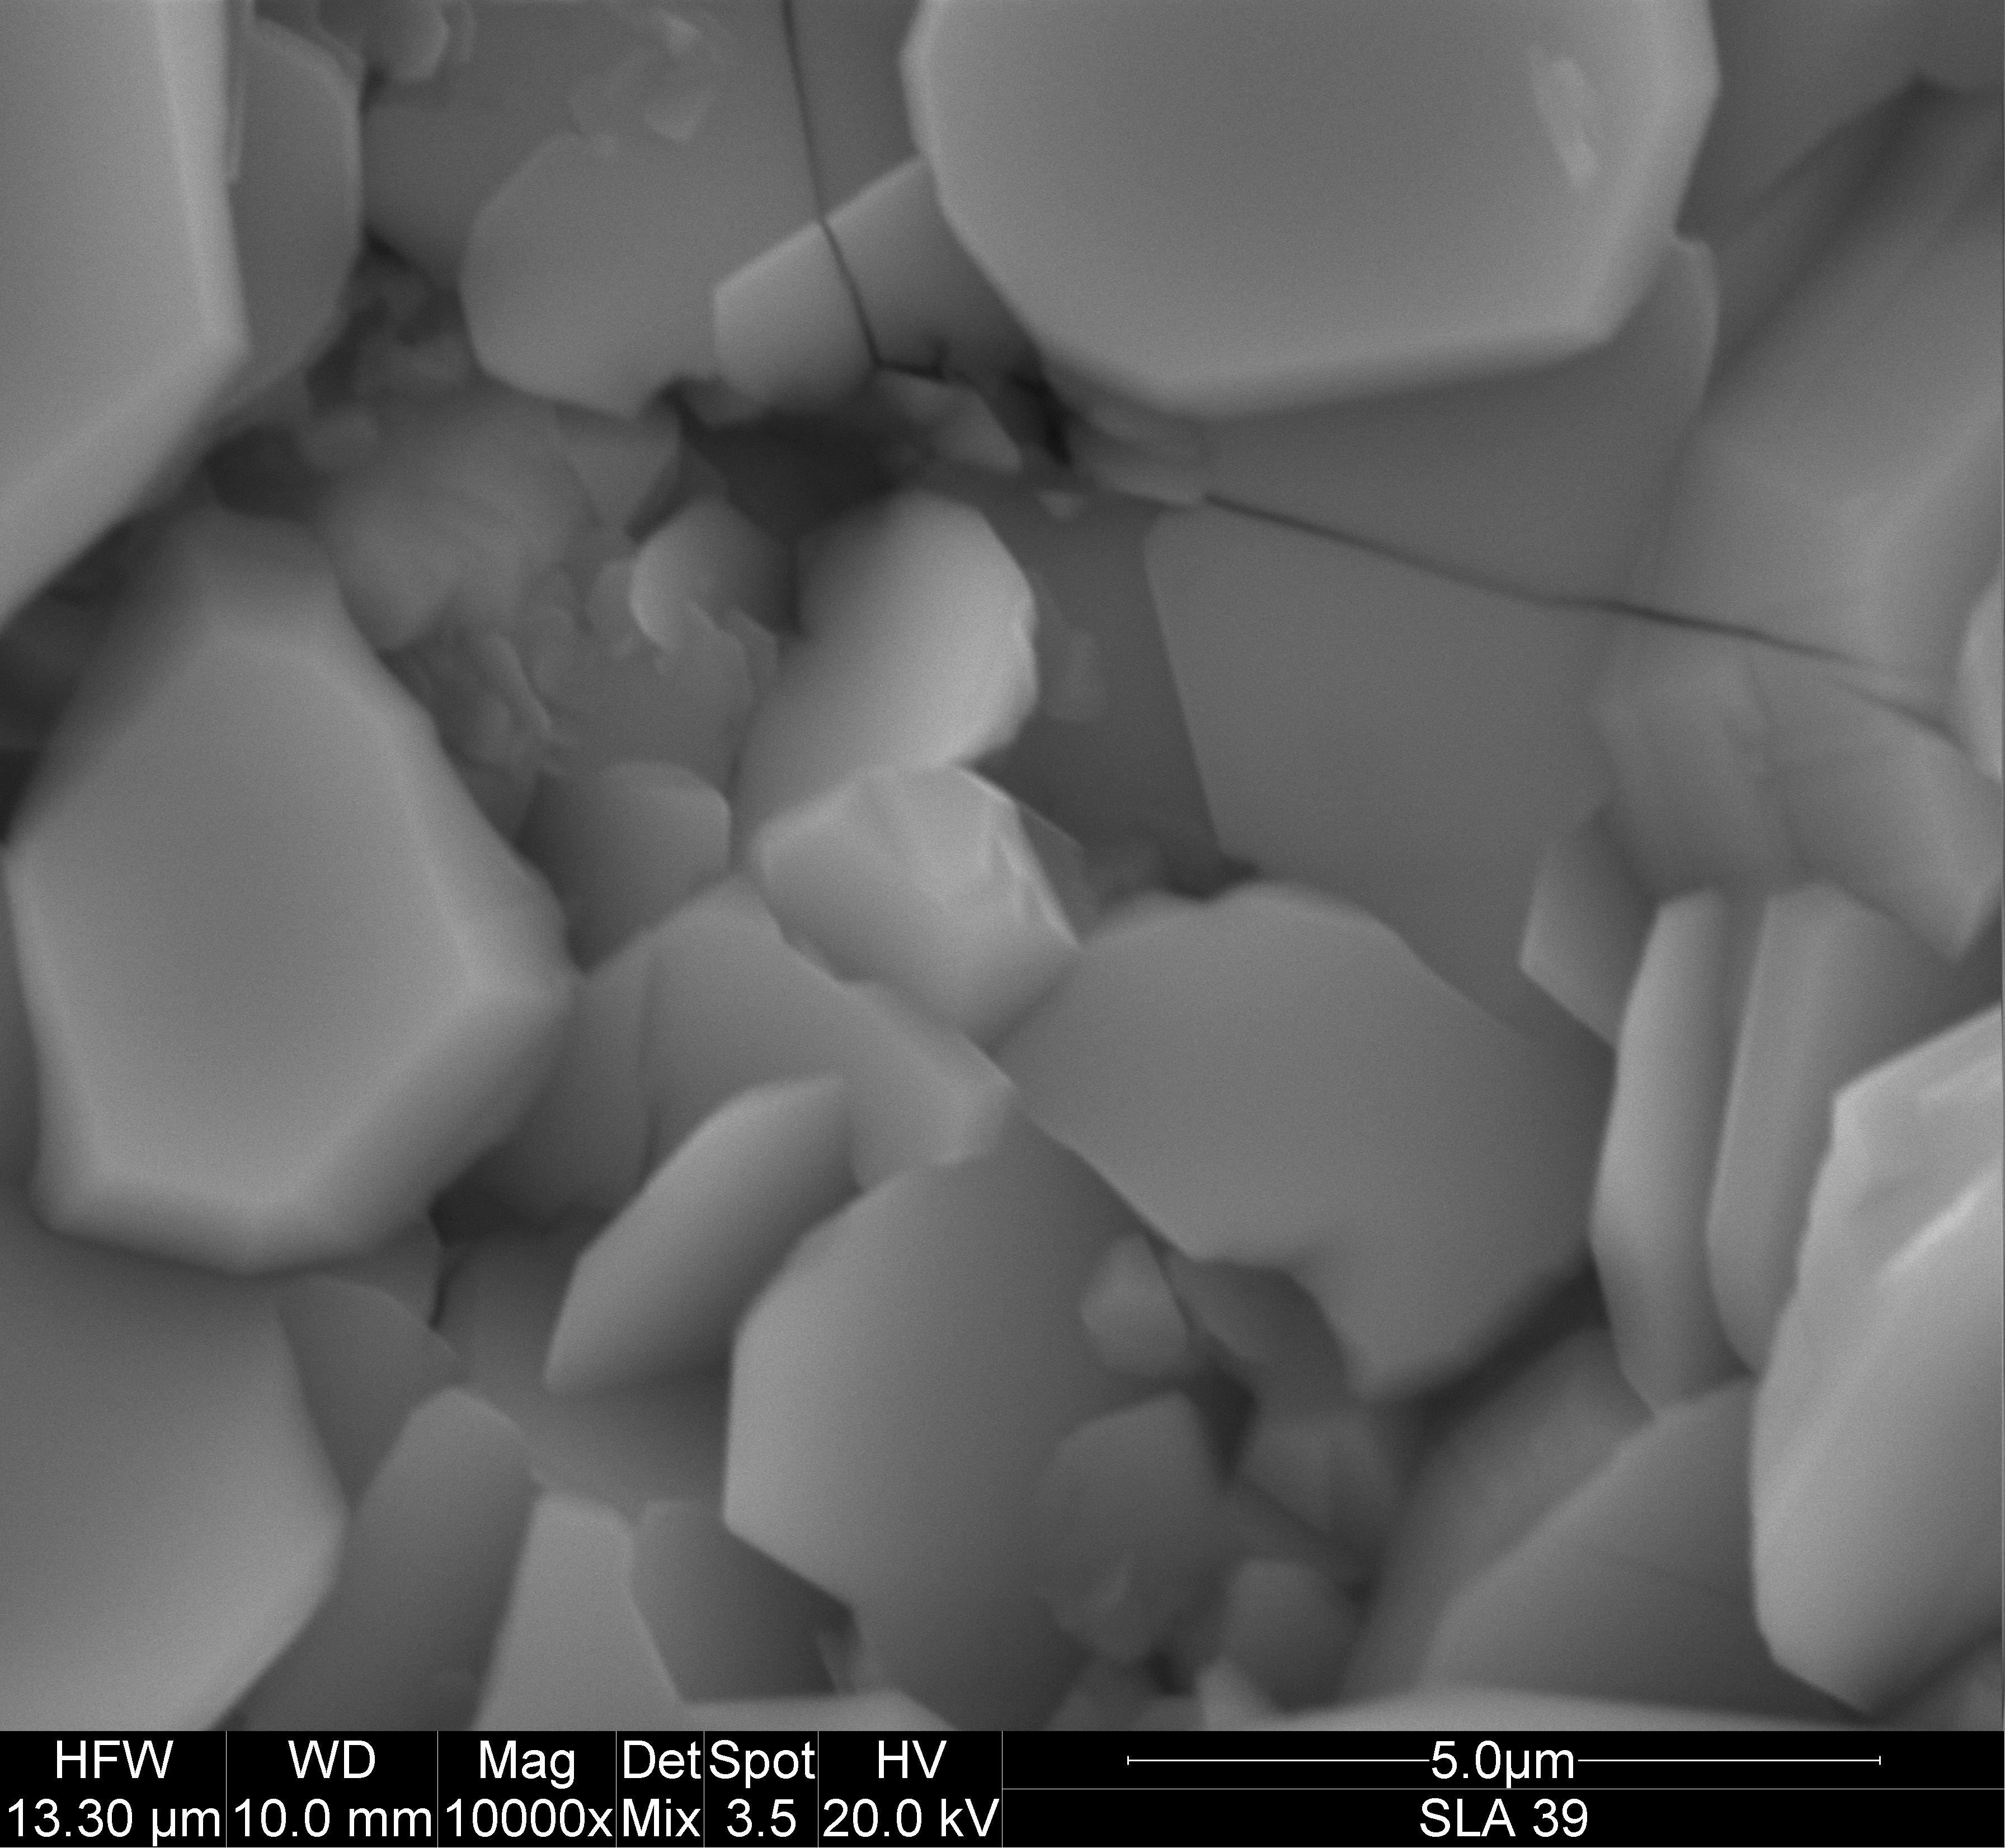
\includegraphics[width=0.8\linewidth]{Wlasciwosci/SLA39_MIX_10000.jpg}} \\b)
	\end{minipage}
	\caption{Na tym rysunku są przedstawione zdjęcia $\alpha'$-$\mathbf{Ga_{2}S_{3}}$ za pomocą SEM przy powiększeniu : a) 5000 razy, b) 10000 razy.[1]}
\end{figure}

Dla wszystkich rysunków, które zostały zrobione za pomocą oprogramowania VESTA, punktem wejściowym są pliki ($\mathbf{CIF}$\footnote{Crystallographic information file (CIF) -- standardowy format pliku tekstowego, służący do zapisu danych krystalograficznych.}).

Poniżej znajduje się zawartość przykładowego pliku ($\mathbf{CIF}$) dla $\alpha'$-$\mathbf{Ga_{2}S_{3}}$:
\begin{lstlisting}
	data_409550-ICSD
	#@2015 by Fachinformationszentrum Karlsruhe, and the U.S. Secretary of 
	#Commerce on behalf of the United States.  All rights reserved.
	_database_code_ICSD                409550
	_audit_creation_date               2002/10/01
	_audit_update_record               2005/04/01
	_chemical_name_systematic          'Digallium Sulfide'
	_chemical_formula_structural       'Ga2 S3'
	_chemical_formula_sum              'Ga2 S3'
	_publ_section_title
	;
	Refinement of the crystal structure of digallium trisulfide, Ga2 S3
	;
	loop_
	_citation_id
	_citation_journal_abbrev
	_citation_year
	_citation_journal_volume
	_citation_page_first
	_citation_page_last
	_citation_journal_id_ASTM
	primary 'Zeitschrift fuer Kristallographie - New Crystal Structures'
	2001 216 327 328 ZKNSFT
	_publ_author_name
	;
	Jones, C.Y.;Bryan, J.C.;Kirschbaum, K.;Edwards, J.G.
	;
	_cell_length_a                     11.107(2)
	_cell_length_b                     6.395(1)
	_cell_length_c                     7.021(1)
	_cell_angle_alpha                  90.
	_cell_angle_beta                   121.17(3)
	_cell_angle_gamma                  90.
	_cell_volume                       426.7
	_cell_formula_units_Z              4
	_symmetry_space_group_name_H-M     'C 1 c 1'
	_symmetry_Int_Tables_number        9
	_refine_ls_R_factor_all            0.035
	loop_
	_symmetry_equiv_pos_site_id
	_symmetry_equiv_pos_as_xyz
	1	'x, -y, z+1/2'
	2	'x, y, z'
	3	'x+1/2, -y+1/2, z+1/2'
	4	'x+1/2, y+1/2, z'
	loop_
	_atom_type_symbol
	_atom_type_oxidation_number
	Ga3+	3
	S2-	-2
	loop_
	_atom_site_label
	_atom_site_type_symbol
	_atom_site_symmetry_multiplicity
	_atom_site_Wyckoff_symbol
	_atom_site_fract_x
	_atom_site_fract_y
	_atom_site_fract_z
	_atom_site_occupancy
	_atom_site_attached_hydrogens
	Ga1 Ga3+ 4 a 0.04213(8) 0.40234(19) 0.12512(11) 1. 0 
	Ga2 Ga3+ 4 a 0.20026(9) 0.93206(18) 0.11559(13) 1. 0 
	S1 S2- 4 a -.0050(3) 1.0861(4) -.0162(6) 1. 0 
	S2 S2- 4 a 0.3378(3) 0.9075(3) 0.4999(4) 1. 0 
	S3 S2- 4 a 0.1741(3) 0.5840(3) 0.0084(4) 1. 0 
	
	loop_
	_atom_site_aniso_label
	_atom_site_aniso_type_symbol
	_atom_site_aniso_U_11
	_atom_site_aniso_U_22
	_atom_site_aniso_U_33
	_atom_site_aniso_U_12
	_atom_site_aniso_U_13
	_atom_site_aniso_U_23
	Ga1 Ga3+ 0.0068(7) 0.0130(6) 0.0096(7) 0.0007(4) 0.0042(5) 0.0005(4)
	Ga2 Ga3+ 0.0065(7) 0.0133(6) 0.0102(7) -.0003(4) 0.0045(5) -.0012(4)
	S1 S2- 0.0065(12) 0.0160(13) 0.0182(13) -.0001(8) 0.0043(10) -.0048(9)
	S2 S2- 0.0041(12) 0.0153(12) 0.0098(15) -.0009(8) 0.0036(11) -.0019(8)
	S3 S2- 0.0084(13) 0.0121(12) 0.0095(12) -.0017(8) 0.0056(10) -.0010(8)
	#End of data_409550-ICSD
\end{lstlisting}
Pliki cif są generowane podczas badań strukturalnych rentgenowskich materiału. Są w wolnym dostępie. Te pliki są punktem wejściowym do generowania struktur w programie VESTA. Zawartością tego pliku jest:
\begin{itemize}
	\item Informację ogólne o związku;
	\item Miejsce skąd wzięte te informacje;
	\item Parametry komórki elementarnej;
	\item Grupa symetrii;
	\item Położenia atomów w komórce elementarnej. 
\end{itemize} 

\subsection{Własności i zastosowania $\mathbf{Ga_{2}S_{3}}$}
Jednym z najważniejszych problemów materiałów półprzewodnikowych stosowanych w fotoelektronice jest opracowanie związków o stabilnych właściwościach pod wpływem promieniowania UV, promieniowania rentgenowskiego i $\gamma$, a także opracowanie detektorów promieniowania jonizującego w oparciu o te materiały. Strukturalne defekty w materiale wywoływane są pod wpływem promieni UV, promieniowania rentgenowskiego i $\gamma$. Koncentracja i rodzaj tych defektów zależy zarówno od dawki promieniowania, jak i rodzaju materiału. Detektory promieniowania rentgenowskiego i promieniowania UV oparte na tych materiałach muszą spełniać warunek, że koncentracja ich własnych defektów jest znacznie wyższa niż koncentracja defektów wywołanych promieniowaniem. Materiały takie jak $\mathbf{A_{2}^{III}C_{3}^{VI}}$, szczególnie $\mathbf{Ga_{2}S_{3}}$, spełniają to wymaganie. $\frac{1}{3}$ pozycji w podsieci kationowej są nieobsadzone i tworzą luki, czyli defekty kryształu. Koncentracja własnych defektów w tych materiałach wynosi około $10^{22}\;cm^{-3}$. Przewodność elektryczna pojedynczych kryształów $\mathbf{Ga_{2}S_{3}}$ w normalnej temperaturze wynosi około $10^{-12}\;\Omega^{-1}cm^{-1}$. Przewodność elektryczna wzrasta 3 razy z domieszką $\mathbf{Cd}$.[10][15][28]
\subsubsection{Własności}
\begin{enumerate}
	\item Szerokopasmowa światłoczułość w zakresie blue - UV. Takie promieniowanie elektromagnetyczne trafiając na materiał $\mathbf{Ga_{2}S_{3}}$ zmienia jego przewodność elektryczną. Domieszkując ten materiał można wpływać na światłoczułość;
	\item Fotoluminescencja w zakresie green-blue, to odpowiada przedziału energetycznemu 1.60 - 3.00 eV;
	\item Optyczna nieliniowość. $\mathbf{Ga_{2}S_{3}}$ generuje drugą harmoniczną. To znaczy jeżeli na materiał zostanie skierowane promieniowanie o dużej intensywności i monochromatyczności o częstotliwości $2\omega$, to obok promieniowania wychodzącego z tego materiału pojawi się promieniowanie o długości $\omega$.
	\item Wysoka przezroczystość w IR. Czyli materiał nie tłumi promieniowania w podczerwieni.
	\item High damage treshold. Czyli ma dużą odporność na uszkodzenia.
\end{enumerate}

\subsubsection{Zastosowania}

$\mathbf{GaS}$ długi czas zajmował wysoką pozycję wśród materiałów do aplikacji THz. Ma bardzo szerokie okna dla promieniowania o długości fali 0.62 – 20 $\mu m$ i od 50 $\mu m$. Ale jego warstwowa struktura i wynikające z tego słabe właściwości mechaniczne ograniczają możliwości zastosowania tego materiału. $\mathbf{Ga_{2}S_{3}}$ jest przezroczysty dla fal o długości 0.44 – 25 $\mu m$ co jest pokazano na wykresie poniżej:

\begin{figure}[H]
	\begin{center}
		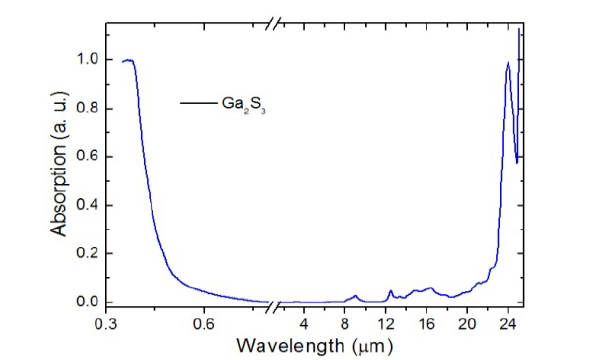
\includegraphics[width=0.8\linewidth]{Wlasciwosci/Widmo-absorpcji-Ga2S3.png}
		\caption{Widmo absorpcji dla $Ga_{2}S_{3}$.[25]}
	\end{center}
\end{figure}

\begin{enumerate}
	\item Materiał $\mathbf{Ga_{2}S_{3}}$ ma zastosowanie optyczne i optoelektroniczne (diody elektroluminescencyjne (LED), absorber UV w fotowoltaicznych urządzeniach, generator drugiej harmonicznej, generator trzeciej harmonicznej np. w materiale $\mathbf{Ti_{2}S}$-$\mathbf{Ga_{2}S_{3}}$-$\mathbf{GeS_{2}}$), ze względu na swoją skośną i szeroką przerwę energetyczną). (duże czyli bulk kryształy) Struktura cienkowarstwowa Ga2S3/In/Ga2S3 ma potencjalne zastosowanie jako rezonator mikrofalowy. Jego dwójłomność 0,025 jest większa niż $\mathbf{CdSe}$, która pozwala dopasować fazę SHG dla długości fali dłuższej niż 1910 $\mu m$. [22]][26]
	
	\item Kolejne z możliwych zastosowań tego materiału jest pasywacja powierzchni półprzewodnikowej III - V tj. do utworzenia "natywnej" warstwy siarczkowej na $\mathbf{GaAs}$ lub $\mathbf{InP}$ poprzez siarkowanie na powierzchni; tak, że rekombinacja powierzchni $\mathbf{GaAs}$ lub $\mathbf{InP}$ można radykalnie stłumić, co z kolei znacząco poprawia wydajność urządzenia W dziedzinie nauki o materiałach i technologii brakuje skutecznych warstw pasywacji powierzchniowej  dla $\mathbf{GaAs}$.[30][33]
	
	\item Materiały $\mathbf{GaS}$ i $\mathbf{Ga_{2}S_{3}}$ mają doskonałe właściwości dla soczewek optycznych, optycznych amplifikacji do telekomunikacji i produkcji laserowej i są nietoksyczne.[20][29]
\end{enumerate}

\newpage

\subsection{Widmo ramanowskie i polaryzacyjne}

Widmo ramanowskie dla związku $\alpha$-$\mathbf{Ga_{2}S_{3}}$ ma 7 pików, które odpowiadają przesunięciom: 1) 119, 2) 135, 3) 148, 4) 238, 5) 309, 6) 331, 7) 392 $cm^{-1}$.

W budowie krystalicznej $\mathbf{Ga_{2}S_{3}}$ występują tetraedry $[\mathbf{GaS_{4}}]$ co skutkuje tym, że widmo ramanowskie $\mathbf{Ga_{2}S_{3}}$ można podzielić na mody wewnętrzne tetraedru $[\mathbf{GaS_{4}}]$ oraz mody związane
z oddziaływaniami zewnętrznymi.


\begin{figure}[H]
	\begin{center}
		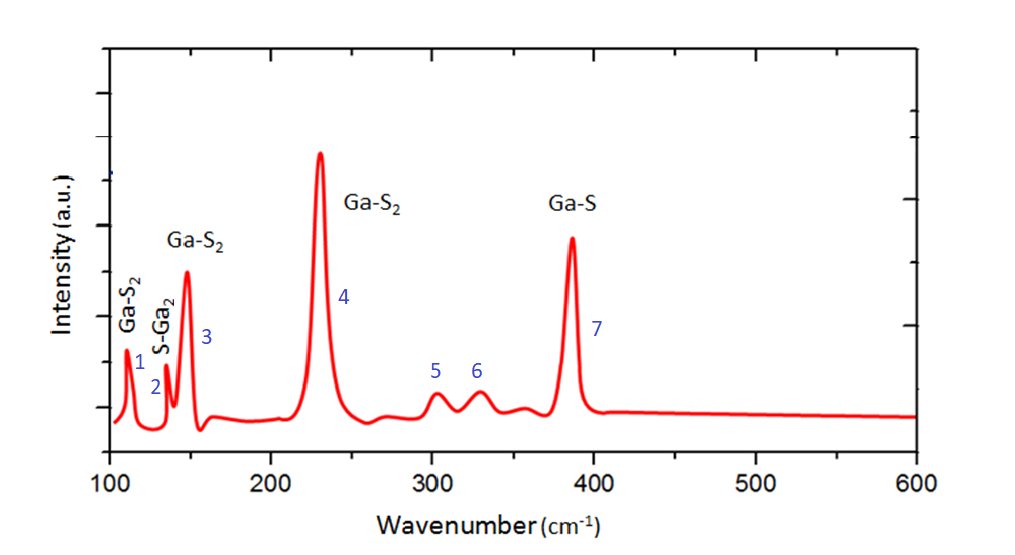
\includegraphics[width=1.0\linewidth]{Wlasciwosci/Raman-Ga2S3.png}
		\caption{Widmo ramanowskie dla $\alpha'$-$\mathbf{Ga_{2}S_{3}}$.[11]}
	\end{center}
\end{figure}

Piki ramanowskie w przedziale 200-450 $cm^{-1}$ są przypisywane drganiom rozciągającym $\mathbf{Ga}$-$\mathbf{S}$. W tym zakresie znajdują się mody A1 i F2. Piki ramanowskie występujące poniżej 200 $cm^{-1}$ są związane z drganiami zginającymi dla tetraedrów $[\mathbf{GaS_{4}}]$. 
W tym zakresie spektralnym występują mody o symetrii E i E2. W zakresie niskich częstości występują również mody translacyjne i rotacyjne dla grup $[\mathbf{GaS_{4}}]$, ale nie są one aktywne ramanowsko. Najbardziej intensywny pik ramanowski dla struktur krystalicznych $\mathbf{Ga_{2}S_{3}}$ jest obserwowany dla około 235 $cm^{-1}$ – jest to mod A1, który jest związany z drganiami siarki w kierunku wakansji galowej. 


W zależności od kierunku polaryzacji światła laserowego, które oddziałuje z fononami w materiale intensywności pików będą się zmieniać. Po zaobserwowaniu tych zmian można uzyskać widmo polaryzacyjne. Przykładowe widmo polaryzacyjne znajduje się poniżej:
 
\begin{figure}[H]
	\begin{center}
		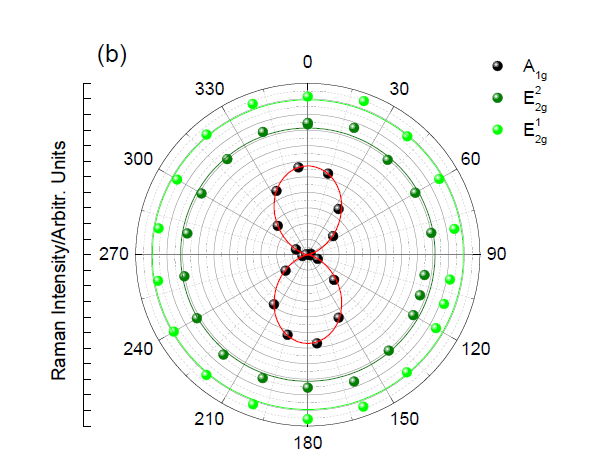
\includegraphics[width=0.8\linewidth]{Wlasciwosci/Spectre-polarization-Ga2S3.png}
		\caption{Przykładowe widmo polaryzacyjne dla trzech pików $\mathbf{A_{1g}}$ $\mathbf{E_{2g}^{2}}$ $\mathbf{E_{2g}^{1}}$. Tu intensywność czyli pole powierzchni piku to odległość od środka do punktu, który odpowiada określonemu kątowi. Ten kąt jest kątem między kierunkiem drgania dipola a promieniowaniem pobudzającym. Widać, że tylko pik $\mathbf{A_{1g}}$ znacząco reaguje na zmianę polaryzacji.[19]}
	\end{center}
\end{figure}

Intensywność piku ramanowskiego można pokazać taką relacją:
\begin{equation}
	I_{s} \sim |e_{i}\mathbf{R}e_{s}|^{2}
\end{equation}
\begin{itemize}
	\item $e_{i}$ i $e_{s}$ - wektory polaryzacji promieniowania podającego i rozproszonego odpowiednio.
	\item $\mathbf{R}$ - Tensor ramanowski, który zależy od symetrii kryształu i konkretnego drgającego modu.
\end{itemize}

Wektor elektryczny rozproszonego światła ramanowskiego jest powiązany z wektorem elektrycznym światła padającego przez charakterystyczny tensor ramanowski. Unikalny tensor ramanowski istnieje dla każdego aktywowanego molekularnego trybu wibracyjnego.

Tensor ramanowski jest macierzą 3 x 3, która łączy wektor elektryczny (x1, y1, z1) promieniowania wzbudzającego z wektorem elektrycznym (x2, y2, z2) promieniowania rozproszonego podanego przez:

\begin{figure}[H]
	\begin{center}
		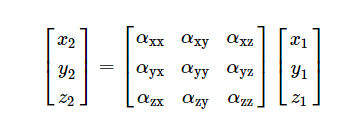
\includegraphics[width=0.5\linewidth]{Wlasciwosci/Raman-Tensor.png}
	\end{center}
\end{figure}

Ponieważ $a_{xy} = a_{yx}$, $a_{yz} = a_{zy}$ i $a_{zx} = a_{xz}$, należy określić tylko sześć składowych tensorowych. W tym przypadku x, y i z są prostokątnymi osiami współrzędnych, które są ustalone na cząsteczce, ale są arbitralnie wybierane. Jeśli główne osie tensora ramanowskiego, które są unikalne dla dowolnego danego pasma ramanowskiego, są wybierane jako układ współrzędnych xyz, to sześć niezerowych składników tensora są zredukowane do trzech elementów diagonalnych: $a_{xx}$, $a_{yy}$ i $a_{zz}$. Tak więc, tensor Ramana może zostać ustalony przez określenie $a_{xx}$, $a_{yy}$ i $a_{zz}$ oraz trzech parametrów kątowych, które ustalają główne osie tensorowe w układzie współrzędnych xyz.

Aby zdefiniować system głównych osi (xyz) lokalnego tensora ramanowskiego, arbitralnie wybieramy trzy nieliniowo ułożone atomy $E_1$, $E_2$ i $A$ w cząsteczce będącej przedmiotem zainteresowania w taki sposób, że oś y jest równoległa do linii łączącej atomy $E_1$ i $E_2$, oś x jest równoległa do linii prostopadłej łączącej atom $A$ z osią y, a oś z jest prostopadła do osi y i x. Chociaż zestaw wybranych osi może nie obejmować całego kąta bryłowego 4$\Pi$, zwykle wystarcza do określenia tensora Ramana. Wynika to z faktu, że każda przerwa między kierunkami dwóch kandydujących osi wprowadza błąd, który jest mały w stosunku do błędów w pomiarach eksperymentalnych.



